\section{Methods}

\subsection{Dataset and Cohort}
We use the UK Biobank (UKB)~\cite{ukbiobank}, a prospective cohort of
500{,}000 UK adults aged 40--69 at recruitment.
We focus on participants with at least one respiratory or pulmonary disease
diagnosis (ICD-10: J09--J98 for diseases of the respiratory system, or
I26--I27 for pulmonary heart disease), extracted from hospital episode
statistics fields (p41202, p41204, p41270).
This subgroup is motivated by evidence that all-cause mortality prediction
is structurally hardest in respiratory multimorbidity cohorts, where
heterogeneous disease trajectories, compounding comorbidity burden, and
highly variable event timing create a particularly demanding pattern
recognition challenge~\cite{ukbmdrmf}.
Further restricting to participants aged $\geq$\,60 at the end of follow-up
or death yields $n\,=\,124{,}158$ participants.
The binary outcome is all-cause mortality after age 60.
We apply a stratified 70/15/15 split: train\,86{,}911,
val\,18{,}624, test\,18{,}623 (event rate 26.2\% in all splits).
Features extracted prior to age 60 include: age at recruitment, sex, BMI,
smoking status, alcohol status, living alone, 21 blood biomarkers
(HbA1c, total cholesterol, HDL/LDL, CRP, cystatin~C, albumin, etc.),
11 binary comorbidity flags (T2 diabetes, CKD, depression, stroke, etc.),
and the full temporal history of ICD-10 diagnoses.

\subsection{Experimental Design}
\label{sec:design}
We design a controlled three-axis ablation to ask:
\emph{how should temporal clinical information be encoded for mortality
risk stratification?}
Figs.~\ref{fig:input_formats} and~\ref{fig:methods} show the full design.

\begin{figure}[t]
  \centering
  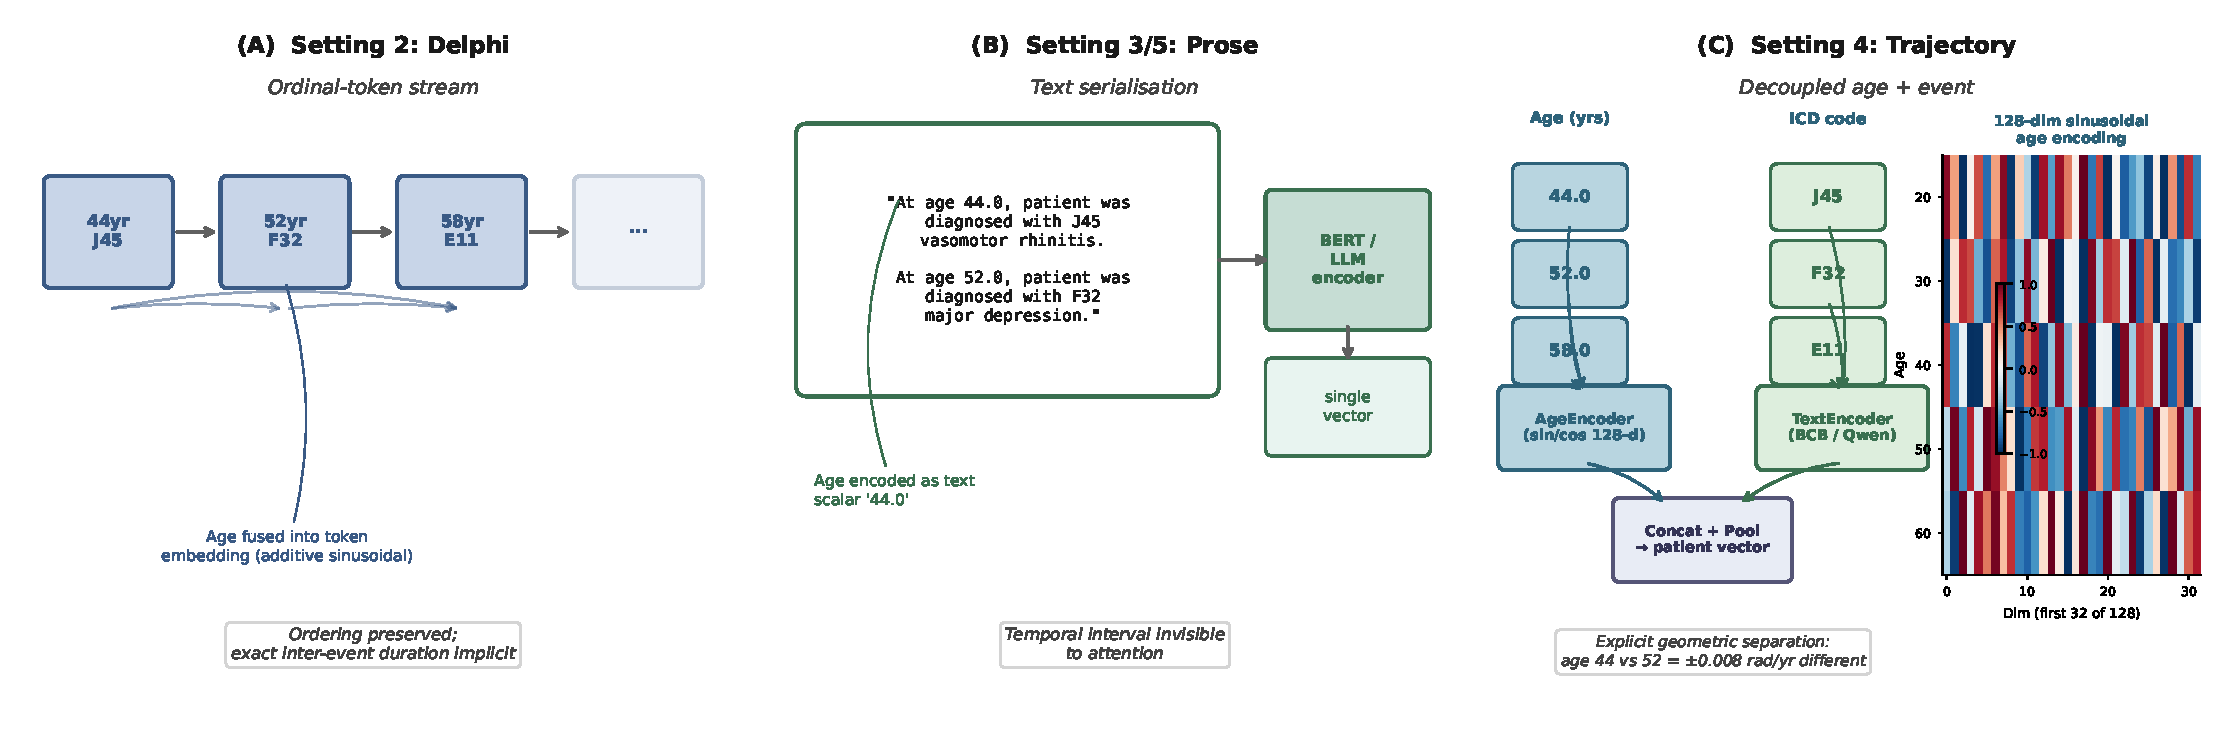
\includegraphics[width=\textwidth]{figures/figure_input_formats}
  \caption{How the five input settings encode temporal information differently.
           (A)~Setting 2 (Delphi): age is fused additively into the token embedding
           via a learned sinusoidal positional encoding; temporal ordering is
           preserved but exact inter-event duration is implicit.
           (B)~Settings 3 and 5 (Prose): age appears as a text scalar
           (\textit{``at age 44.0''}) — invisible as geometry to the encoder's attention.
           (C)~Setting 4 (Trajectory): age and ICD event are encoded in \emph{separate}
           streams (128-dim sinusoidal age encoding; text encoder for the ICD token),
           then concatenated per event and mean-pooled.
           The inset heatmap shows the 128-dim sinusoidal age encoding for ages
           20--60, confirming explicit geometric separation between events at
           different life stages.}
  \label{fig:input_formats}
\end{figure}

\paragraph{Axis A — Input Representation (5 settings).}
Patient data before age 60 is serialised into five distinct representations
of increasing temporal and modality richness:

\begin{enumerate}
  \item \textbf{Cross-sectional (Setting 1).}
        Demographics, 21 biomarkers, and 11 binary comorbidity flags are
        concatenated into a 39-dimensional numeric vector.
        No temporal information and no text encoder are used.
        This corresponds to the standard supervised CoxPH baseline.

  \item \textbf{Sequential ordinal (Setting 2).}
        ICD-10 events before age 60 are encoded as an ordinal token stream
        \textit{``44yr:J45 $\rightarrow$ 52yr:F32 $\rightarrow$ \ldots''}.
        Temporal ordering is captured but exact durations between events are
        implicit.
        This is the input format consumed by Delphi~\cite{delphi2024},
        a generative transformer pre-trained on longitudinal EHR event
        sequences, which we evaluate in zero-shot mode.

  \item \textbf{Isolated temporal prose (Setting 3).}
        The same ICD events are serialised as natural-language sentences:
        \textit{``At age 44.0, patient was diagnosed with J45 vasomotor
        rhinitis.''}\
        Demographics and biomarkers are provided as a separate numeric
        feature block and fused with the embedding at evaluation time.

  \item \textbf{Decoupled time and event (Setting 4).}
        Age at diagnosis and the ICD token are encoded in parallel, separate
        streams: the age is mapped to a 128-dim sinusoidal encoding adapted
        from the Transformer positional encoding~\cite{vaswani2017attention}
        (matching Delphi's AgeEncoding~\cite{delphi2024}), and each ICD token string is
        embedded independently by the chosen text encoder.
        Per-event representations are concatenated (age $\parallel$ token)
        and mean-pooled across all events.
        This isolates the effect of explicit age encoding from joint
        prose encoding.

  \item \textbf{Unified summary prose (Setting 5).}
        All four modalities are combined into a single paragraph:
        demographics, lab values with units, comorbidity flags, and disease
        history in chronological prose.
        This is the only setting in which numeric biomarker values are
        included directly in the text.
        \emph{No raw numeric features are concatenated at evaluation time};
        the embedding alone is fed to CoxPH.
\end{enumerate}

\paragraph{Axis B — Encoder Architecture (Settings 3--5).}
Settings 3, 4, and 5 require a text encoder.
We compare two frozen encoders to test whether results are specific to one
model family:
\begin{itemize}
  \item \textbf{Qwen3-Embedding (8B)}~\cite{qwen3}: a general-purpose
        sentence-embedding model with 4096-dim output,
        last-token pooling, and 8192-token context (supports all five settings
        with no truncation).
  \item \textbf{Bio\_ClinicalBERT}~\cite{bioclinicalbert}: a 110M-parameter
        BERT model pre-trained on MIMIC-III clinical notes.
        Mean-pooled 768-dim output; hard max-length of 512 tokens.
        For Setting 5 (unified summary prose), texts may exceed 512 tokens,
        causing truncation of the disease-history tail, which we report as a
        limitation.
\end{itemize}
In Setting 4, the token embedder within the decoupled pipeline is swapped
between Qwen3-8B and Bio\_ClinicalBERT; the sinusoidal age encoding is
shared across both variants.

\paragraph{Axis C — Feature Fusion (Settings 3--4 only).}
Settings 3 and 4 produce a dense embedding that must be combined with the
39-dim raw feature block.
We compare two linear fusion methods:
\begin{itemize}
  \item \textbf{Concatenation (concat)}: the embedding is PCA-compressed
        to 64 dims (fit on training set), then appended to the standardised
        raw features to form a 103-dim input for CoxPH.
        This is the standard late-fusion baseline.
  \item \textbf{Element-wise summation (sum)}: the embedding is
        PCA-projected to match the raw feature width $d$, both blocks are
        independently standardised (train statistics only), zero-padded to a
        common width, and added element-wise.
        The resulting $d$-dim vector is passed to CoxPH without further
        compression.
        This tests whether additive fusion in a shared feature space improves
        over concatenation.
\end{itemize}

\paragraph{Resulting experiment matrix.}
Combining Settings 1--2 (no encoder, no fusion) with the 2-encoder $\times$
2-fusion ablation for Settings 3--4 and 2-encoder for Setting 5 gives
\textbf{12 total cells} (Table~\ref{tab:matrix}).

\begin{table}[ht]
\centering
\small
\caption{Experiment matrix. Settings 1 and 2 have no encoder or fusion axis.
         BCB = Bio\_ClinicalBERT.
         Qwen3-8B embedding runs used an NVIDIA RTX 3090; BCB embedding runs
         (cells marked $\star$) used an NVIDIA RTX 4090 (remote server).}
\label{tab:matrix}
\begin{tabular}{llcc}
\toprule
Setting & Encoder & Fusion & Cell \\
\midrule
S1 — Cross-sectional      & —           & —      & Baseline CoxPH \\
S2 — Sequential ordinal   & Delphi      & —      & Delphi zero-shot \\
\midrule
S3 — Isolated prose       & Qwen3-8B    & concat & S3·Qwen·concat \\
S3 — Isolated prose       & Qwen3-8B    & sum    & S3·Qwen·sum \\
S3 — Isolated prose       & BCB$^\star$ & concat & S3·BCB·concat$^\star$ \\
S3 — Isolated prose       & BCB$^\star$ & sum    & S3·BCB·sum$^\star$ \\
\midrule
S4 — Decoupled time+event & Qwen3-8B    & concat & S4·Qwen·concat \\
S4 — Decoupled time+event & Qwen3-8B    & sum    & S4·Qwen·sum \\
S4 — Decoupled time+event & BCB$^\star$ & concat & S4·BCB·concat$^\star$ \\
S4 — Decoupled time+event & BCB$^\star$ & sum    & S4·BCB·sum$^\star$ \\
\midrule
S5 — Unified prose        & Qwen3-8B    & —      & S5·Qwen \\
S5 — Unified prose        & BCB$^\star$ & —      & S5·BCB$^\star$ \\
\bottomrule
\end{tabular}
\end{table}

\subsection{Evaluation Protocol}
We report five metrics on the held-out test set:
(i) Harrell C-index (concordance, higher is better)~\cite{harrellcindex};
(ii) mean time-dependent AUC (TD-AUC) averaged over horizons
    9.5, 15.4, and 19.7 years (higher is better);
(iii) Integrated Brier Score (IBS, lower is better), measuring calibration;
(iv) \emph{Restricted mean survival time} (RMST): per-patient
    $\int_0^\tau S(t\mid x)\,\mathrm{d}t / 365.25$ (in years), restricted
    to $\tau = $ the 80th-percentile follow-up horizon, computed via
    trapezoidal integration over a 100-point survival curve.
    RMST provides an interpretable calibration complement to IBS,
    capturing whether the model's predicted life-years align with
    the observed restricted mean under the Kaplan--Meier estimator.
(v) \emph{Bootstrap confidence intervals:} 1{,}000 paired resamples of the test set to compute 95\% CIs for C-index and paired difference $p$-values for key contrasts (S4 vs.\ S3, S4 vs.\ S1, S5 vs.\ S1).
All metrics are computed with \texttt{lifelines} and \texttt{scikit-survival}.
No information leakage: PCA projections (both axes B and C) and CoxPH
coefficients are fitted on training splits only; val and test transforms
use the training-fit parameters.

\begin{figure}[t]
  \centering
  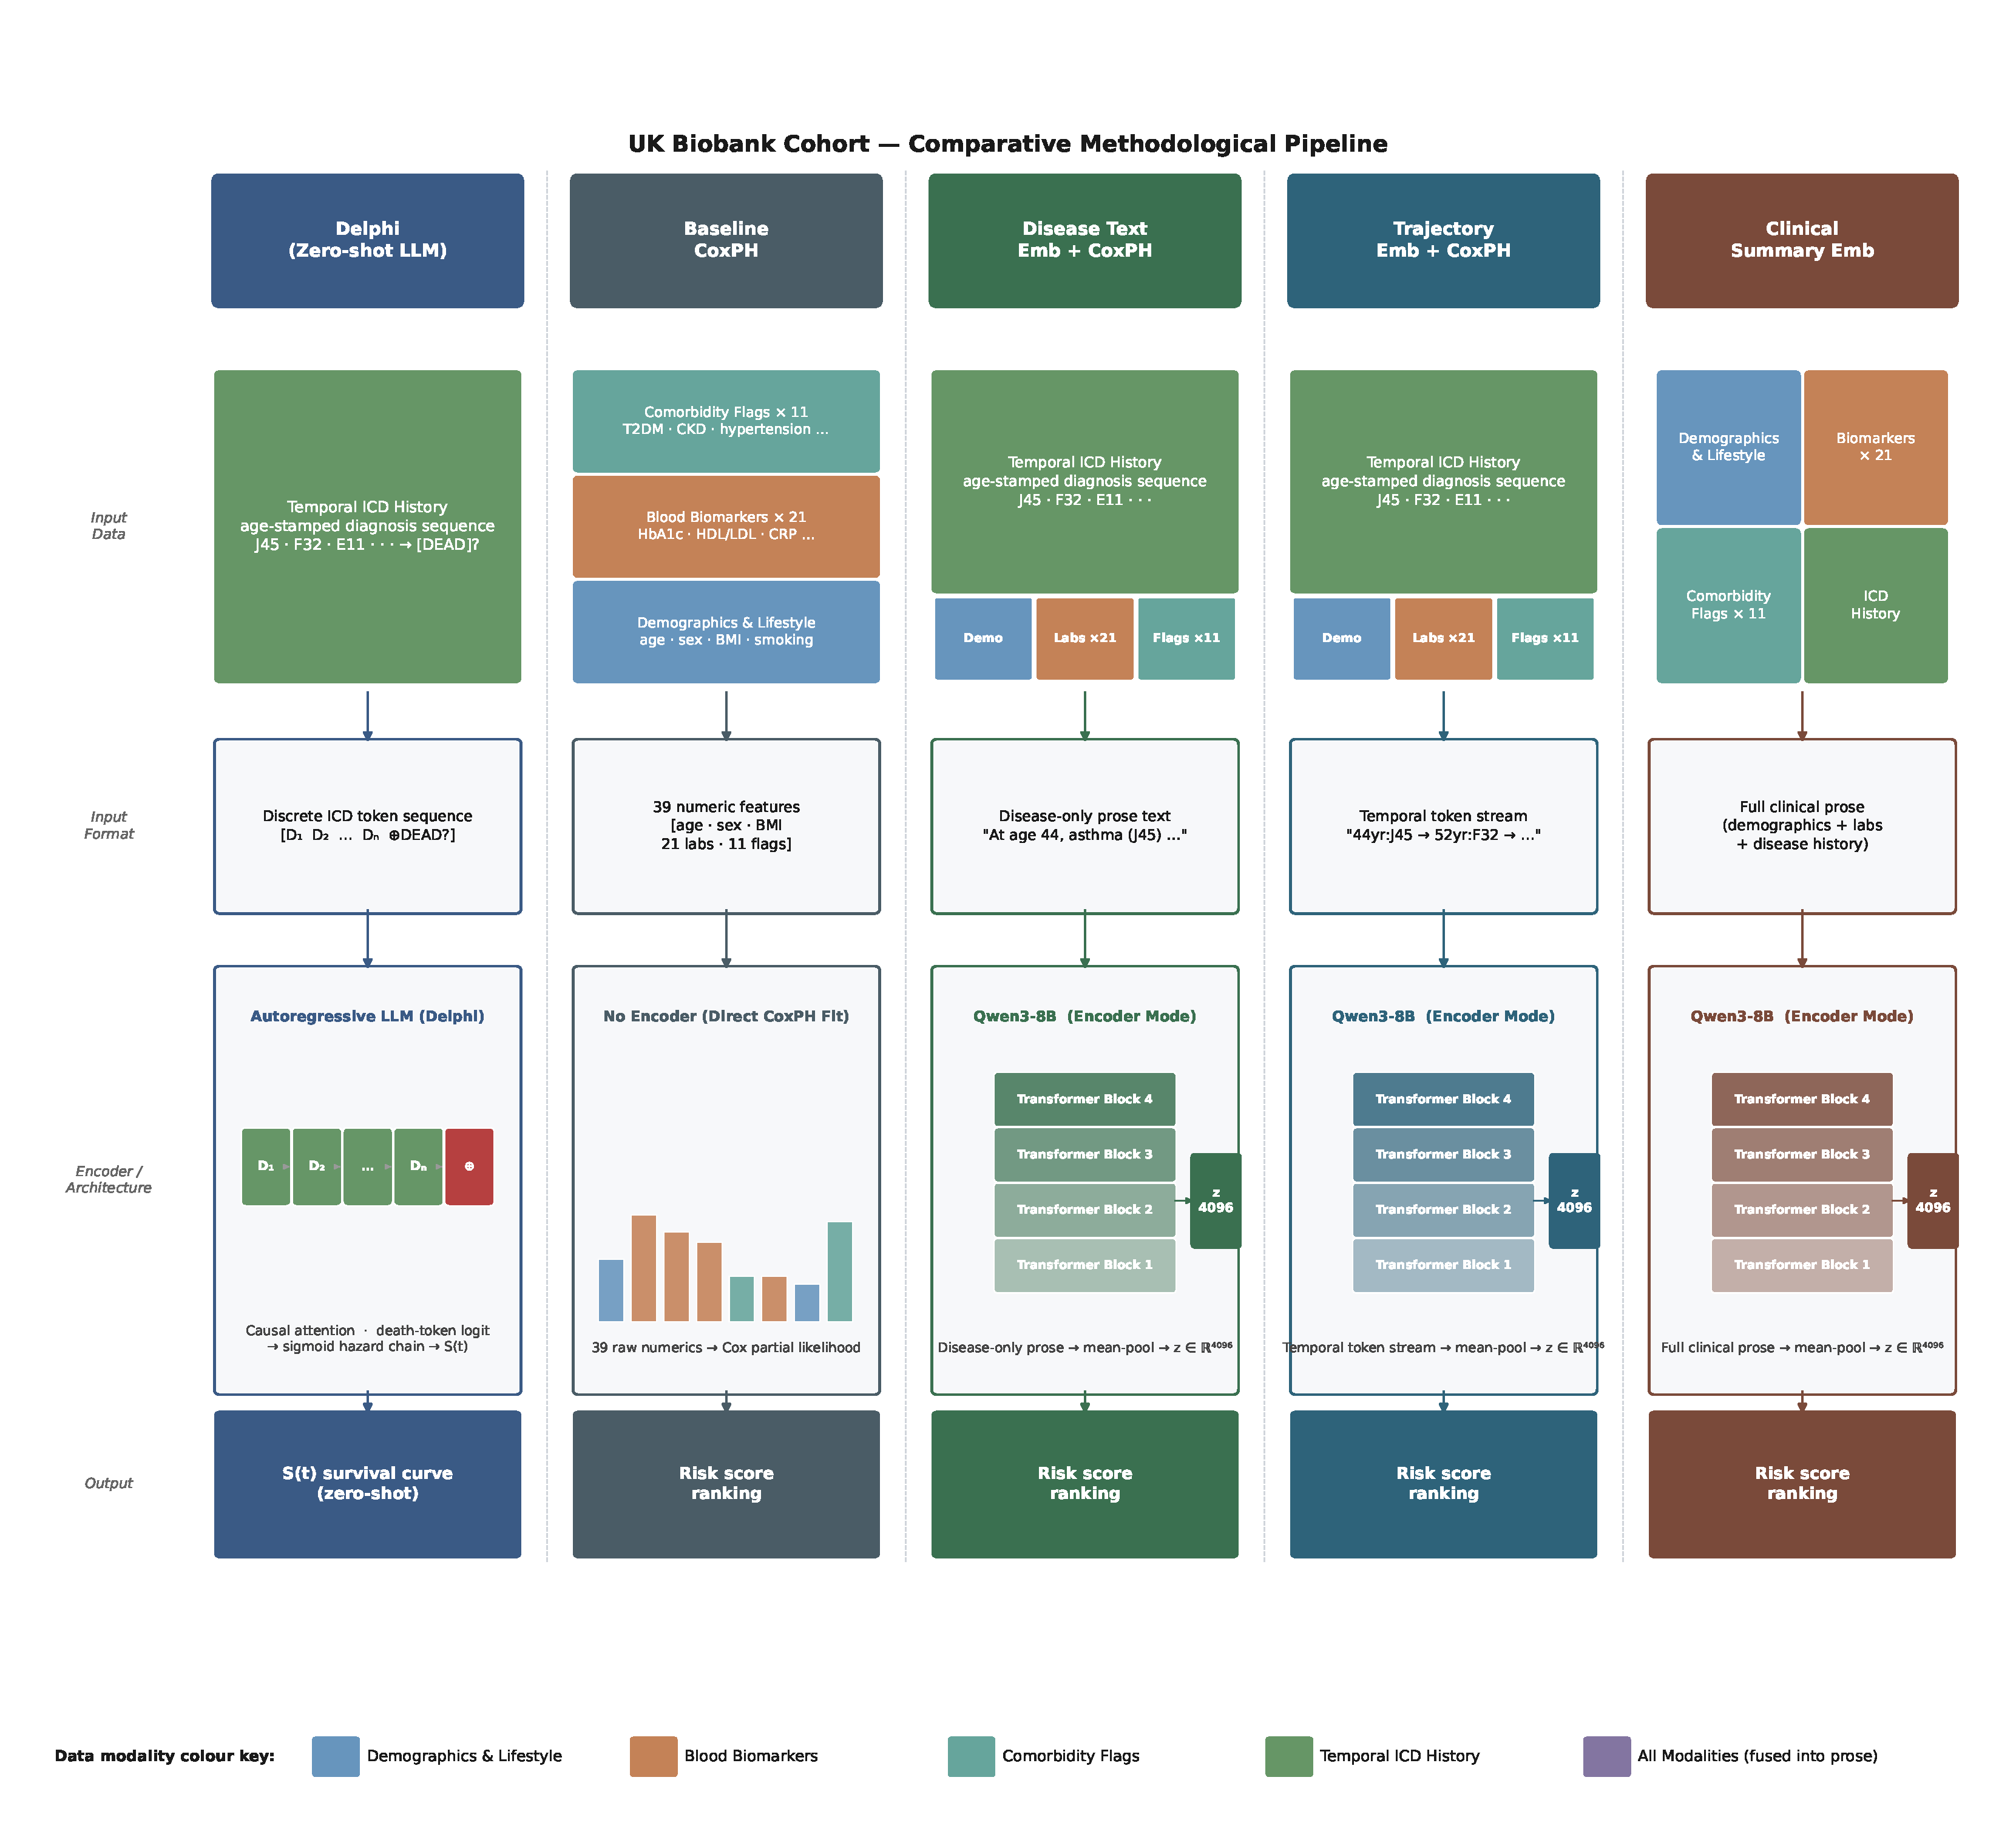
\includegraphics[width=\textwidth]{figures/figure_methods}
  \caption{Architecture overview. Patient data is separated into five modalities
           and routed through three axes: (A) five input representations
           (see also Fig.~\ref{fig:input_formats} for a detailed comparison of
           temporal encoding strategies), (B) two encoder architectures for
           settings 3--5, and (C) two fusion methods for settings 3--4.}
  \label{fig:methods}
\end{figure}
